\documentclass{standalone}
\usepackage{tikz}
\usepackage{amsmath}
\usepackage{amssymb}
\usetikzlibrary{decorations.markings, arrows.meta}

\begin{document}
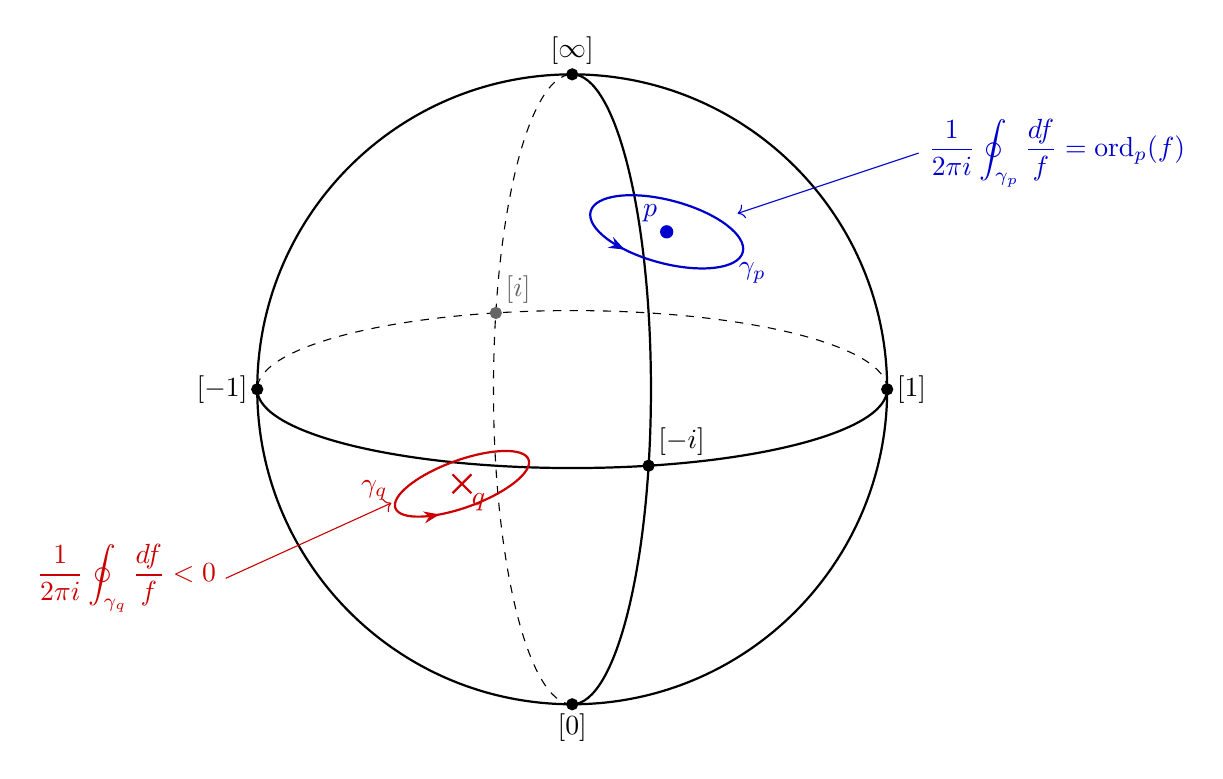
\begin{tikzpicture}[scale=2]
	% Draw the Riemann Sphere (CP^1)
%	\shade[ball color=white, opacity=0.8] (0,0) circle (2cm);
%	\draw[thick] (0,0) circle (2cm);
	
%	% Draw the equator to give 3D perspective
%	\draw[dashed, draw=black!60] (2,0) arc (0:180:2cm and 0.5cm);
%	\draw[thick, draw=black!60] (2,0) arc (0:-180:2cm and 0.5cm);
%	\draw[dashed, draw=black!60] (0,-2) arc (270:-90:0.5cm and 2cm);
%	\draw[thick, draw=black!60] (0,2) arc (90:-90:0.5cm and 2cm);
%	\node[left, font=\large] at (-2, 1.2) {$\mathbb{CP}^1\simeq\mathbb C\cup\{\infty\}$};
	
	
	\draw[thick] (0,0) circle (2);
	\draw[thick] (-2,0) arc[start angle=180,end angle=360,x radius=2,y radius=0.5];
	\draw[dashed] (2,0) arc[start angle=0,end angle=180,x radius=2,y radius=0.5];
	\draw[thick] (0,-2) arc[start angle=-90,end angle=90,x radius=0.5,y radius=2];
	\draw[dashed] (0,-2) arc[start angle=270,end angle=90,x radius=0.5,y radius=2];
	
	
	% --- Point p (e.g., a zero) ---
	\coordinate (P) at (0.6, 1.0);
	\fill[blue!80!black] (P) circle (1.2pt) node[above left] {$p$};
	
	% Contour \gamma_p around p
	\begin{scope}[shift={(P)}, rotate=-15]
		\draw[thick, blue!80!black, 
		decoration={markings, mark=at position 0.65 with {\arrow{Stealth[length=2mm]}}}, 
		postaction={decorate}] 
		(0,0) ellipse (0.5cm and 0.2cm);
		\node[blue!80!black, right] at (0.45, -0.15) {$\gamma_p$};
	\end{scope}
	
	% Equation annotation for p
	\draw[->, blue!80!black, shorten >=3pt] (2.2, 1.5) -- (1.0, 1.1);
	\node[right, blue!80!black] at (2.2, 1.5) {$\displaystyle \frac{1}{2\pi i}\oint_{\gamma_p}\frac{df}{f} = \text{ord}_p(f)$};
	
	% --- Point q (e.g., a pole) ---
	\coordinate (Q) at (-0.7, -0.6);
	% Mark pole with a cross
	\draw[red!80!black, thick] (Q) +(-0.06,-0.06) -- +(0.06,0.06);
	\draw[red!80!black, thick] (Q) +(-0.06,0.06) -- +(0.06,-0.06);
	\node[red!80!black, below right] at (Q) {$q$};
	
	% Contour \gamma_q around q
	\begin{scope}[shift={(Q)}, rotate=20]
		\draw[thick, red!80!black, 
		decoration={markings, mark=at position 0.65 with {\arrow{Stealth[length=2mm]}}}, 
		postaction={decorate}] 
		(0,0) ellipse (0.45cm and 0.15cm);
		\node[red!80!black, left] at (-0.4, 0.1) {$\gamma_q$};
	\end{scope}
	
	% Equation annotation for q
	\draw[->, red!80!black, shorten >=3pt] (-2.2, -1.2) -- (-1.1, -0.7);
	\node[left, red!80!black] at (-2.2, -1.2) {$\displaystyle \frac{1}{2\pi i}\oint_{\gamma_q}\frac{df}{f} < 0$};
	
	\filldraw[black] (0,2) circle (1pt) node[above] {$[\infty]$};
	\filldraw[black] (0,-2) circle (1pt) node[below] {$[0]$};
	\filldraw[black] (-2,0) circle (1pt) node[left] {$[-1]$};
	\filldraw[black] (2,0) circle (1pt) node[right] {$[1]$};
	\filldraw[black] (.485,-.485) circle (1pt) node[above right] {$[-i]$};
	\filldraw[black!60] (-.485,.485) circle (1pt) node[above right] {$[i]$};
	
%	% --- Principal Divisor Summary ---
%	\node[align=center, fill=white, draw=black!30, rounded corners, inner sep=6pt] at (0, -2.8) {
%		\textbf{Principal Divisor} \\[4pt]
%		$\displaystyle (f) = \sum_{x \in \mathbb{CP}^1} \left(\frac{1}{2\pi i}\oint_{\gamma_x}\frac{df}{f}\right) \cdot [x]$
%	};
	
\end{tikzpicture}
\end{document}